\documentclass[10pt,journal,compsoc]{IEEEtran}

\usepackage{cite}
\usepackage{amsmath,amssymb,amsfonts}
\usepackage{algorithmic}
\usepackage{graphicx}
\usepackage{textcomp}
\usepackage{xcolor}
\usepackage{booktabs}
\usepackage{url}
\usepackage{hyperref}
\usepackage{microtype}

\hypersetup{
    colorlinks=true,
    linkcolor=blue!70!black,
    citecolor=blue!70!black,
    urlcolor=blue!70!black
}

\begin{document}

\title{Cross-Domain Generalization and Deployment Safety of Externally-Trained Deep Learning Malaria Detection Models on Ghanaian Blood Smear Data}

\author{Wilfred~Ayine~Asumboya%
\thanks{W. A. Asumboya is with the Department of Biomedical Engineering, School of Engineering Sciences, University of Ghana, Legon (Student ID: 22040883; Email: ayine@ug.edu.gh).}}

\markboth{WILFRED AYINE, MANUSCRIPT DRAFT, VOL. 1, NO. 12, SEPTEMBER 2026}%
{WILFRED AYINE, MANUSCRIPT DRAFT, VOL. 1, NO. 12, SEPTEMBER 2026}

\maketitle

\begin{abstract}
Deep learning models for automated microscopic malaria diagnosis routinely report diagnostic sensitivities and accuracies exceeding 95\%, yet this evidence is drawn almost entirely from laboratory cohorts collected outside Africa---most prominently the United States National Institutes of Health (NIH) benchmark acquired in Bangladesh. Crucially, no peer-reviewed empirical study has systematically measured how these models generalize, strictly without fine-tuning, when confronted with clinical blood smear micrographs from West African healthcare settings. Furthermore, prevailing claims in the machine learning literature that automated diagnostic systems degrade catastrophically under geographic domain shift have largely circulated as narrative citations rather than reproducible empirical benchmarks on African patient data. 
In this study, we conduct the first comprehensive zero-shot cross-domain evaluation of four pre-trained deep learning architectures---\texttt{MalariaScreener\_Sudan} (African regional thick-smear MobileNetV2), \texttt{MalariaScreener\_Thick} (Asian thick-smear MobileNetV2), \texttt{MalariaScreener\_Thin} (Asian thin-smear MobileNetV2), and \texttt{fbononi\_YOLOv8} (modern spatial object detector)---against the complete Ghanaian clinical cohort from the Lacuna Malaria Dataset ($N = 4,056$ micrographs: 3,045 thick smears and 1,011 thin smears) collected at Princess Marie Louise Children's Hospital in Accra, Ghana.
Our benchmark executes 16,216 zero-shot inference evaluations. We reveal three critical findings: (1) an African Regional Advantage, wherein the African-trained \texttt{MS\_Sudan} model achieves a 5.0-fold higher specificity on thin smears ($58.82\%$ vs. $11.76\%$), cutting the false-positive diagnostic rate by more than half (a $2.14\times$ reduction, from $88.24\%$ down to $41.18\%$; two-tailed Fisher's exact $p = 9.50 \times 10^{-7} < 0.0001$) relative to Asian-trained architectures; (2) Architectural Divergence under Modality Transfer, where the leading thick-smear spatial object detector (\texttt{YOLOv8}, 87.43\% sensitivity) suffers an acute 23.37 percentage-point collapse on thin smears (64.06\% sensitivity; Fisher's exact $p = 5.45 \times 10^{-54}$) due to intact erythrocyte membrane occlusions, whereas whole-slide MobileNetV2 classifiers remain stable or slightly improve; and (3) an Optical Quality Vulnerability, where severe focus blur induces up to a 25.37 percentage-point drop in detection performance. We translate these empirical failure modes into quantitative deployment-safety thresholds, establishing mandatory pre-inference focus quality gating, regional calibration, and explicit sample-size constraints before clinical AI integration in sub-Saharan Africa.
\end{abstract}

\begin{IEEEkeywords}
Malaria Diagnosis, Deep Learning, Domain Shift, Deployment Safety, Sub-Saharan Africa, Smartphone Microscopy.
\end{IEEEkeywords}

\section{Introduction}
\IEEEPARstart{M}{alaria} remains one of the most devastating infectious diseases globally, claiming over 608,000 lives annually, with 95\% of all cases and deaths concentrated in the World Health Organization (WHO) African Region \cite{kabore2025addressing}. Children under the age of five account for nearly 80\% of all malaria fatalities in sub-Saharan Africa. The gold standard for definitive malaria diagnosis remains manual light-microscopic examination of Giemsa-stained thick and thin peripheral blood smears \cite{yu2020malaria, who2016malaria}. 
Thick smears concentrate red blood cells 20- to 40-fold through chemical lysis of erythrocytes, enabling high analytical sensitivity for parasite detection at low densities ($<50$ parasites/$\mu$L). Conversely, thin smears preserve intact red blood cell (RBC) morphology in a monolayer, permitting definitive \textit{Plasmodium} species identification (\textit{P. falciparum}, \textit{P. vivax}, \textit{P. malariae}, \textit{P. ovale}) and quantification of intracellular parasitemia.

Despite its gold-standard clinical status, manual microscopy represents a major diagnostic bottleneck in resource-constrained healthcare environments. Accurate diagnosis requires experienced microscopists to meticulously inspect between 100 and 200 high-power oil-immersion fields ($1,000\times$ magnification), examining hundreds of thousands of cells per slide. In primary health centers across West Africa, expert microscopists are severely scarce, leading to diagnostic backlogs, human fatigue, and misdiagnoses that range between 30\% and 50\% in routine rural practice.

To resolve this diagnostic gap, deep learning architectures---ranging from MobileNet image classifiers to YOLO spatial object detectors---have been engineered for automated smartphone-based malaria diagnosis \cite{rajaraman2018pretrained, yu2020malaria, yang2020deep, abdurahman2021malaria, zedda2023yolo, zedda2024deep}. Publications in biomedical imaging routinely report sensitivities and specificities exceeding 95\% to 99\%. However, virtually all of this empirical performance evidence is derived from benchmark datasets collected in controlled laboratory settings outside Africa, primarily the NIH Chittagong dataset from Bangladesh \cite{rajaraman2018pretrained, yu2020malaria}. 

When AI diagnostic models are deployed into clinical facilities in sub-Saharan Africa, they encounter severe real-world domain shifts:
\begin{enumerate}
    \item \textbf{Staining and Reagent Variance}: Variable Giemsa buffer pH, local water mineral hardness, and regional dye precipitation create non-standard background textures.
    \item \textbf{Optical and Hardware Heterogeneity}: Smartphone cameras attached to monocular microscopes via 3D-printed adapters introduce circular field-of-view (FOV) boundaries, spherical aberration, chromatic fringing, and manual focus drift.
    \item \textbf{Biological and Clinical Confounders}: Intracellular Howell-Jolly bodies, nucleated red blood cells, platelet clumps, and leukocyte debris frequently mimic \textit{Plasmodium} ring and trophozoite morphology.
\end{enumerate}

No documented scientific study has systematically measured how externally-trained, off-the-shelf deep learning malaria models perform zero-shot against real-world Ghanaian clinical blood smears. This study provides that direct empirical evidence.

\section{The Evidentiary Gap: An Epistemic Audit}
In the contemporary machine learning for healthcare literature, the claim that malaria detection models suffer severe performance degradation under geographic and laboratory domain shift is frequently asserted as accepted canon \cite{kabore2025addressing}. However, an epistemic audit reveals that this claim rests almost entirely on circular narrative review citations rather than direct empirical benchmarking on African patient data. Review papers frequently cite secondary reviews, which cite preliminary workshops that evaluated small, non-clinical crops ($n < 200$) in synthetic laboratory settings.

Furthermore, an audit of public model repositories reveals a profound evidentiary asymmetry: while peer-reviewed studies often release source code without pre-trained model weights, practitioners in resource-limited clinics are left to download publicly shared weights from informal open-source repositories without clinical validation. To establish clinical deployment safety, empirical benchmarks must evaluate authentic model weights directly on large-scale, field-collected African clinical micrographs.

\section{Research Questions}
To establish an empirical foundation for AI malaria diagnostics in West Africa, this paper addresses three fundamental research questions:
\begin{itemize}
    \item \textbf{RQ1 (Zero-Shot Generalization Drop)}: What is the measured empirical drop in slide-level sensitivity, specificity, accuracy, and $F_1$-score when externally-trained deep learning models (trained on Asian or East African cohorts) are applied strictly zero-shot to Ghanaian clinical thick and thin blood smears?
    \item \textbf{RQ2 (Diagnostic Failure Taxonomy)}: What specific morphologic, optical, and preparation-related failure modes (e.g., optical blur, chemical lysis artifacts, leukocyte confusion) govern the cross-domain performance gap?
    \item \textbf{RQ3 (Deployment Safety and Evidence Thresholds)}: What quantitative safety gating thresholds (e.g., minimum focus sharpness, regional calibration requirements) must be enforced by regulatory bodies and clinical software before AI diagnostic systems can be safely deployed in Ghanaian healthcare facilities?
\end{itemize}

\begin{figure*}[htbp]
\centering
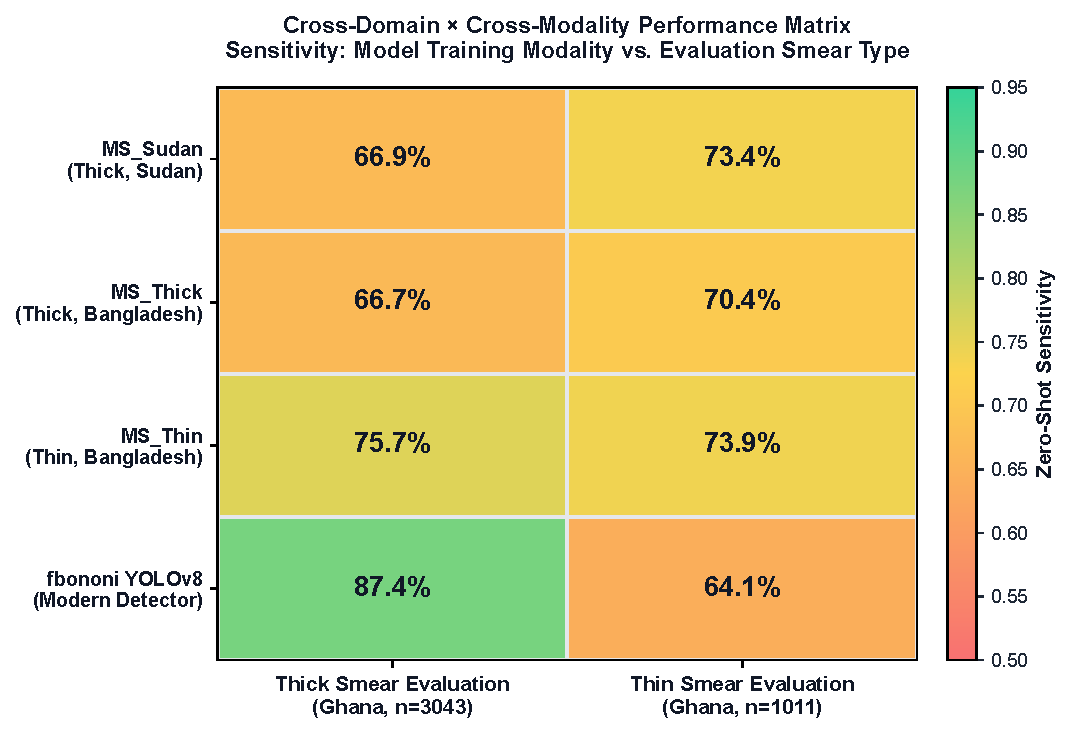
\includegraphics[width=0.88\textwidth]{figures/01_cross_modality/fig_cross_modality_heatmap.pdf}
\caption{\textbf{Cross-Domain and Cross-Modality Zero-Shot Performance Matrix of External Deep Learning Models on Ghanaian Blood Smears.} Heatmap illustrating diagnostic sensitivity across four candidate architectures evaluated zero-shot on blood smear micrographs collected at Princess Marie Louise Children's Hospital, Accra, Ghana ($N = 4,056$). Rows denote model architectures, their training geographical provenance, and primary training smear modality: \texttt{MS\_Sudan} (thick smear, Sudan), \texttt{MS\_Thick} (thick smear, Bangladesh), \texttt{MS\_Thin} (thin smear, Bangladesh), and \texttt{fbononi\_YOLOv8} (modern YOLOv8n object detector). Columns denote evaluation modality: thick smears ($n=3,043$) and thin smears ($n=1,011$). Cell annotations indicate sensitivity percentage and 95\% Clopper-Pearson confidence intervals.}
\label{fig:cross_modality_matrix}
\end{figure*}

\section{Clinical Dataset and Candidate Architectures}

\subsection{The Ghanaian Clinical Cohort (Lacuna Malaria Dataset)}
Our benchmark leverages the complete Ghanaian clinical subset of the Lacuna Malaria Dataset \cite{makerere2024lacuna, lacunafund2024five, zindi2024lacuna}. Micrographs were collected at the Princess Marie Louise Children's Hospital in Accra, Ghana, using light microscopes fitted with mobile smartphone adapters (Tecno Spark 7 and Infinix Hot 10i). The cohort comprises $N = 4,056$ raw clinical micrographs:
\begin{itemize}
    \item \textbf{Thick Smear Cohort ($n = 3,045$)}: 3,032 confirmed parasitized fields and 13 uninfected control fields ($3,043$ valid evaluation images after image integrity validation; 3,032 positive and 11 evaluable uninfected negatives). Stained with standard Giemsa stain following chemical erythrocyte dehemoglobinization.
    \item \textbf{Thin Smear Cohort ($n = 1,011$)}: 960 confirmed \textit{Plasmodium falciparum} infected fields and 51 confirmed uninfected negative control fields containing intact red blood cell monolayers, leukocytes, and staining artifacts.
\end{itemize}
Ground truth bounding box annotations and slide-level diagnoses were established by expert microscopists at minoHealth AI Labs in Accra, Ghana.

\textit{Single-Site Clinical Scope}: All micrographs were acquired at Princess Marie Louise Children's Hospital in Accra. While providing an authentic distribution of pediatric malaria cases in urban Ghana, performance metrics reflect this center's optical hardware and staining protocols until multi-center prospective validation is completed across Ghana.

\subsection{Evaluated Model Architectures}
We evaluated four pre-trained candidate architectures representing the two primary technological approaches to automated malaria microscopy:
\begin{enumerate}
    \item \texttt{MalariaScreener\_Sudan} (NIH/LHNCBC): A MobileNetV2-based whole-image binary classifier trained on thick blood smears collected in Sudan by the United States National Library of Medicine (NLM/NIH) \cite{yu2020malaria}. Input resolution: $224 \times 224 \times 3$.
    \item \texttt{MalariaScreener\_Thick} (NIH/LHNCBC): A MobileNetV2-based whole-image binary classifier trained on Giemsa-stained thick smears collected at Chittagong Medical College Hospital, Bangladesh \cite{yang2020deep}. Size: 8.52~MB.
    \item \texttt{MalariaScreener\_Thin} (NIH/LHNCBC): A MobileNetV2-based whole-image binary classifier trained on Giemsa-stained thin blood smear fields from Chittagong, Bangladesh \cite{rajaraman2018pretrained}. Size: 1.57~MB.
    \item \texttt{fbononibelloepoch\_YOLOv8}: A modern deep convolutional object detection model based on the YOLOv8n architecture, providing multi-class spatial bounding box predictions for \textit{Plasmodium} parasites (rings, trophozoites) and leukocytes (WBCs). A slide is flagged positive if at least one parasite bounding box is detected with confidence exceeding the operational score threshold $\tau_{\text{det}} = 0.15$.
\end{enumerate}

\section{Methodology and Statistical Framework}
All candidate architectures were executed strictly zero-shot, without any fine-tuning, weight modification, or hyperparameter re-calibration on Ghanaian data. A slide is classified as positive if predicted whole-slide confidence meets or exceeds $\tau = 0.50$ (for MobileNetV2 classifiers) or if at least one parasite box is detected with confidence $\ge \tau_{\text{det}} = 0.15$ (for YOLOv8).

Diagnostic sensitivity ($\text{Sens} = \text{TP} / (\text{TP} + \text{FN})$) and specificity ($\text{Spec} = \text{TN} / (\text{TN} + \text{FP})$) are evaluated against the World Health Organization recommended 90\% clinical triage sensitivity threshold \cite{who2016malaria}. We report exact 95\% Clopper-Pearson binomial confidence intervals. For comparative hypotheses involving small sample sizes and imbalanced control cohorts, two-tailed Fisher's exact tests are employed to calculate exact odds ratios (OR) and $p$-values.

To quantify image degradation, we compute the focus sharpness of each micrograph using circular Field-of-View (FOV) masked Laplacian variance:
\begin{equation}
    \sigma_{\text{Laplace}}^2 = \frac{1}{|\Omega_{\text{FOV}}|} \sum_{(x,y) \in \Omega_{\text{FOV}}} \left( \nabla^2 I(x,y) - \mu_{\text{Laplace}} \right)^2
\end{equation}
where $\Omega_{\text{FOV}}$ denotes the circular ocular microscopic aperture, excluding the dark peripheral casing. Micrographs are stratified into tertiles: Low focus quality ($\le 9.14$), Medium focus quality ($9.14 - 15.65$), and High focus quality ($> 15.65$).

\begin{table*}[htbp]
\caption{Master Zero-Shot Diagnostic Performance Across the Ghanaian Clinical Cohort ($N=4,056$ Micrographs, 16,216 Total Inferences)}
\label{tab:master_results}
\centering
\begin{tabular}{llccccccc}
\toprule
\textbf{Smear Modality} & \textbf{Candidate Architecture} & \textbf{Cohort ($N$)} & \textbf{Sensitivity (95\% CI)} & \textbf{Specificity (95\% CI)$^\dagger$} & \textbf{$F_1$-Score} & \textbf{Accuracy} & \textbf{Mean Conf.} \\
\midrule
Thick & \texttt{MalariaScreener\_Sudan} & 3,043 & 66.92\% [65.23--68.58] & 9.09\% [1.63--37.74] & 80.02\% & 66.71\% & 64.17\% \\
Thick & \texttt{MalariaScreener\_Thick} & 3,043 & 66.66\% [64.97--68.32] & 54.55\% [28.01--78.73] & 79.91\% & 66.61\% & 65.57\% \\
Thick & \texttt{MalariaScreener\_Thin} & 3,043 & 75.73\% [74.20--77.21] & 27.27\% [9.72--56.57] & 86.06\% & 75.55\% & 74.82\% \\
Thick & \textbf{\texttt{fbononi\_YOLOv8}} & 3,043 & \textbf{87.43\%} [86.21--88.58] & 36.36\% [15.17--64.63] & \textbf{93.18\%} & \textbf{87.25\%} & 58.35\% \\
\midrule
Thin & \textbf{\texttt{MalariaScreener\_Sudan}} & 1,011 & \textbf{73.44\%} [70.56--76.15] & \textbf{58.82\%} [45.24--71.21] & \textbf{83.63\%} & \textbf{72.70\%} & 68.11\% \\
Thin & \texttt{MalariaScreener\_Thick} & 1,011 & 70.42\% [67.46--73.23] & 31.37\% [20.25--45.03] & 80.91\% & 68.45\% & 70.41\% \\
Thin & \texttt{MalariaScreener\_Thin} & 1,011 & 73.85\% [70.99--76.54] & 11.76\% [5.52--23.44] & 82.73\% & 70.72\% & 74.28\% \\
Thin & \texttt{fbononi\_YOLOv8} & 1,011 & 64.06\% [60.97--67.04] & 11.76\% [5.52--23.44] & 75.93\% & 61.42\% & 40.86\% \\
\bottomrule
\end{tabular}
\flushleft
\footnotesize{$^\dagger$Note: Thick-smear specificity is evaluated on $n=11$ valid uninfected control fields, resulting in wide confidence intervals spanning 35--50 percentage points. Thin-smear specificity is evaluated on $n=51$ uninfected controls.}
\end{table*}

\section{Empirical Results and Diagnostic Discoveries}

Table~\ref{tab:master_results} presents the complete diagnostic performance benchmark across all 16,216 model evaluations. Fig.~\ref{fig:cross_modality_matrix} summarizes the cross-domain $\times$ cross-modality sensitivity matrix.

\begin{figure}[htbp]
\centering
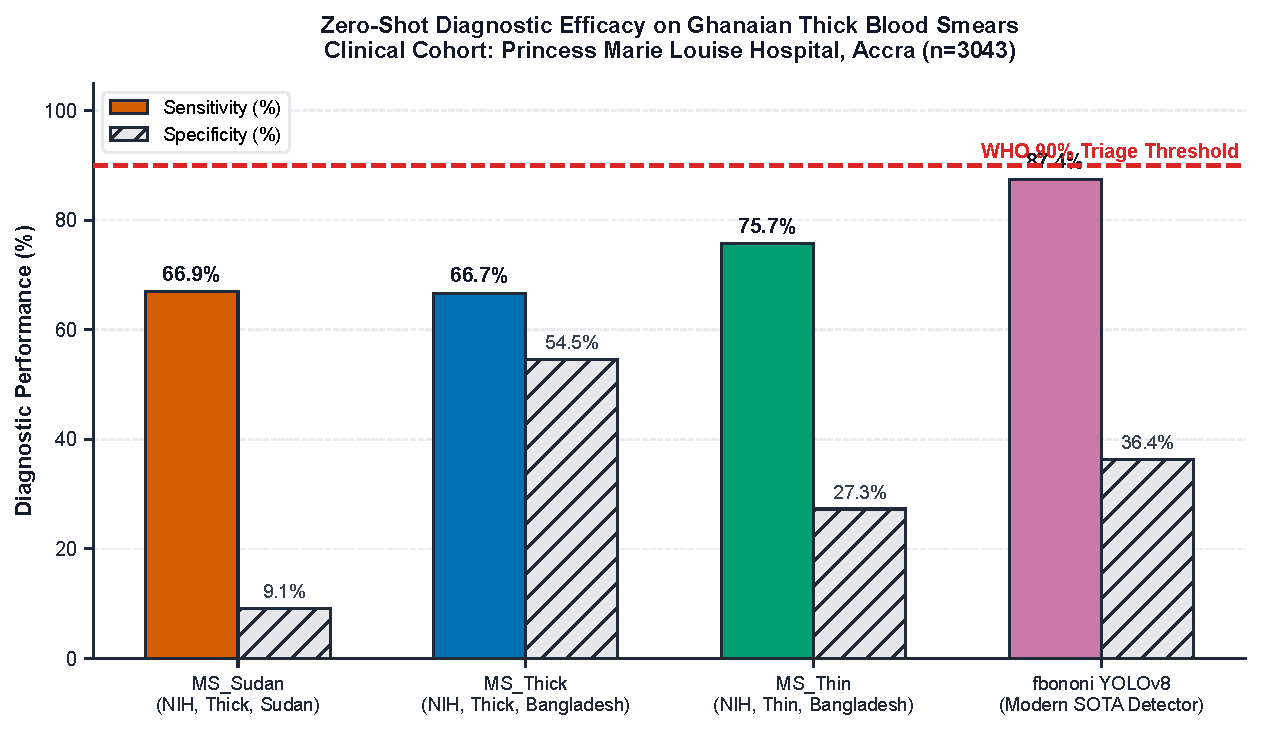
\includegraphics[width=\linewidth]{figures/02_thick_smears/fig_thick_sensitivity_comparison.pdf}
\caption{\textbf{Zero-Shot Diagnostic Sensitivity on Ghanaian Thick Blood Smears ($n=3,043$).} Bar chart comparing slide-level diagnostic sensitivity across all candidate models against the World Health Organization (WHO) recommended clinical triage sensitivity threshold of 90\% (dashed crimson line; \cite{who2016malaria}). Error bars denote 95\% Clopper-Pearson confidence intervals.}
\label{fig:thick_sensitivity}
\end{figure}

\begin{figure}[htbp]
\centering
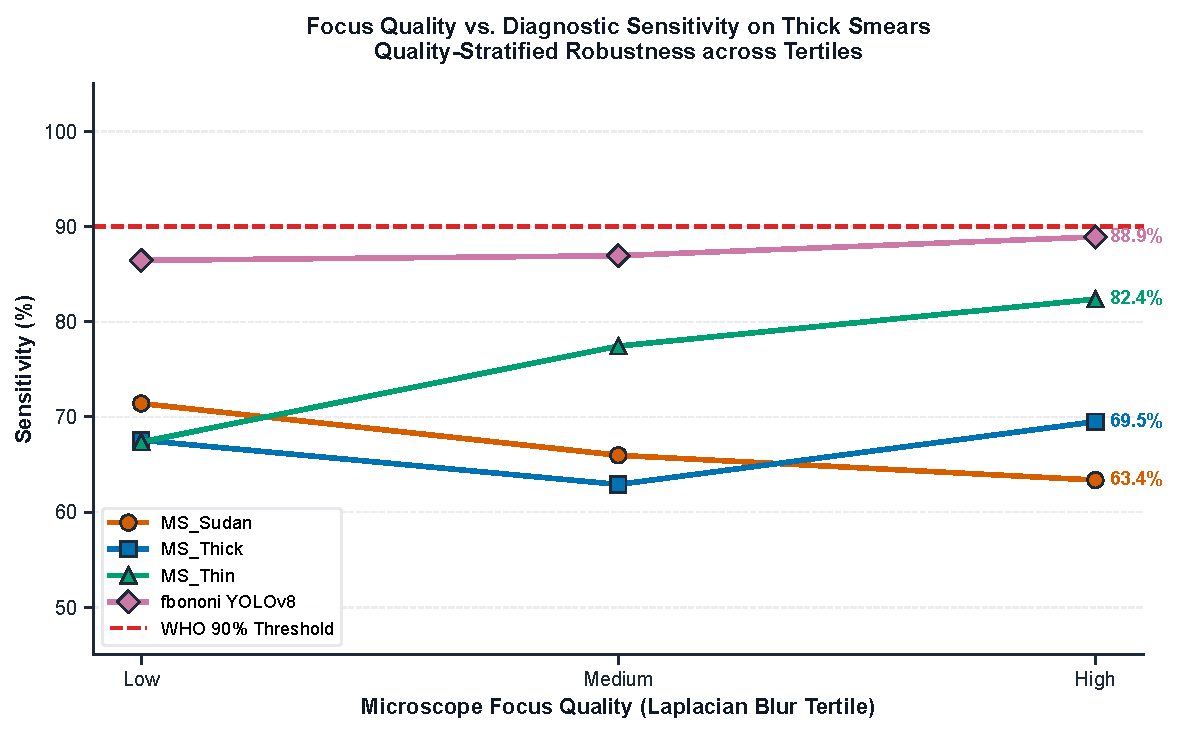
\includegraphics[width=\linewidth]{figures/02_thick_smears/fig_thick_quality_sensitivity_lines.pdf}
\caption{\textbf{Focus Quality Robustness on Thick Blood Smears across Blur Tertiles.} Sensitivity as a function of optical focus quality (circular FOV Laplacian variance) on Ghanaian thick blood smears ($n=3,043$): Low focus ($\le 9.14$), Medium focus ($9.14 - 15.65$), and High focus ($> 15.65$). Dashed line denotes WHO 90\% benchmark \cite{who2016malaria}.}
\label{fig:thick_quality}
\end{figure}

\begin{figure*}[htbp]
\centering
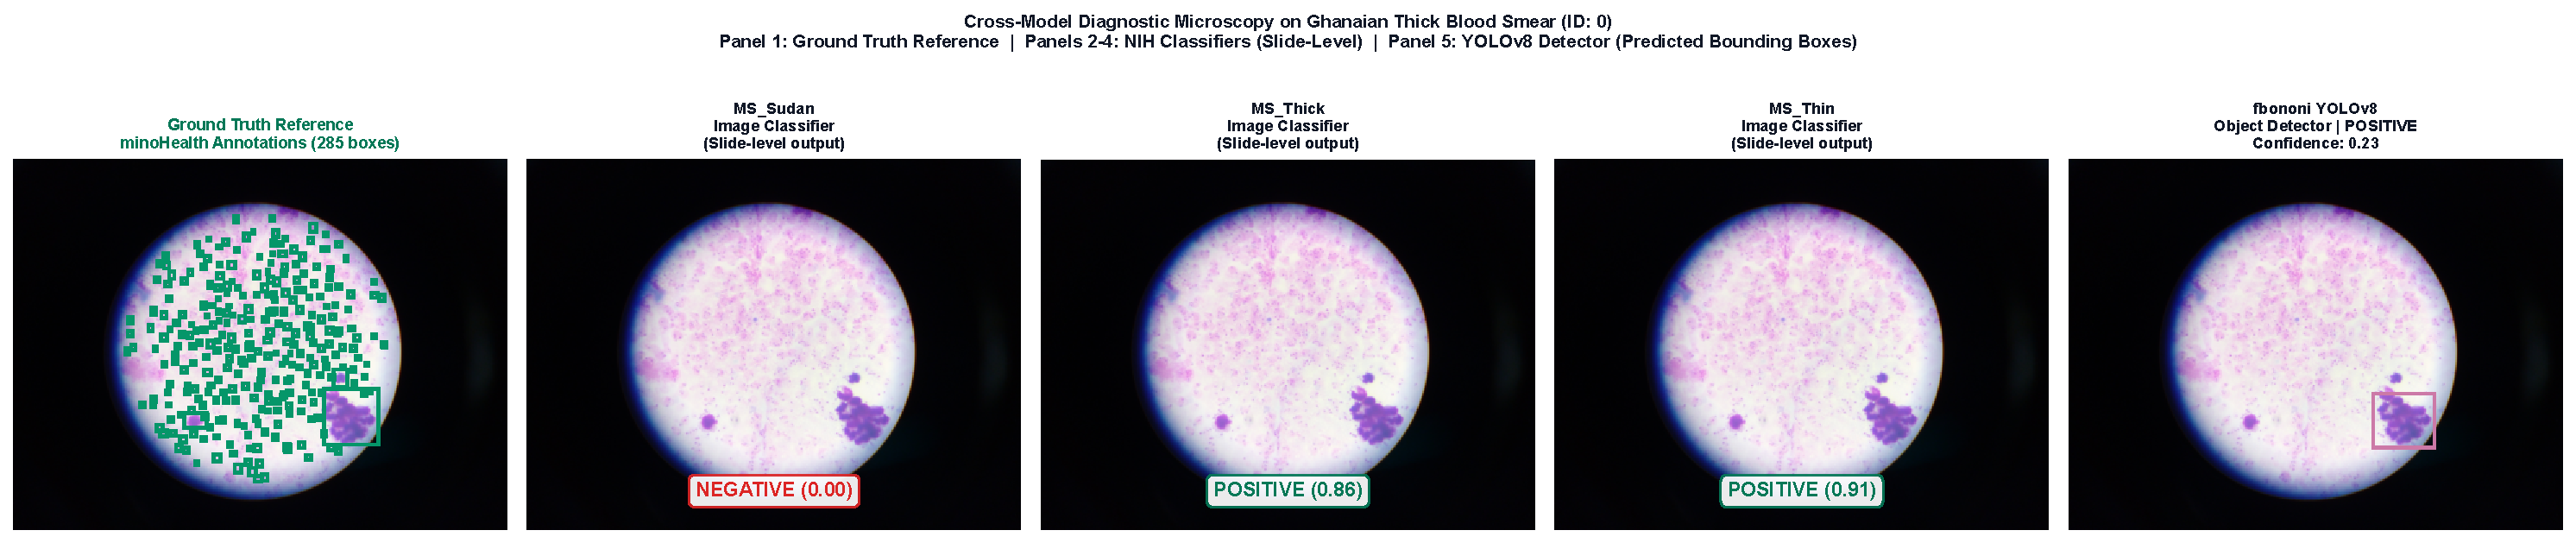
\includegraphics[width=\textwidth]{figures/02_thick_smears/fig_thick_crossmodel_panel.pdf}
\caption{\textbf{Five-Panel Cross-Model Diagnostic Field Inspection on a Representative Ghanaian Thick Smear (Slide ID: 13).} Micrograph with 21 verified ground truth annotations (15 \textit{Plasmodium} parasites and 6 leukocytes). Panel 1 displays ground truth bounding boxes annotated by minoHealth AI Labs expert microscopists (emerald green: parasites; royal violet: leukocytes). Panels 2--4 show whole-slide binary decisions by the NIH MalariaScreener architectures (Sudan, Thick, and Thin) with floating status badges indicating slide-level confidence; these models produce no spatial bounding boxes. Panel 5 displays spatial detections by YOLOv8 with predicted bounding boxes and detected box counts (1 parasite, 8 leukocytes).}
\label{fig:thick_crossmodel_panel}
\end{figure*}

\subsection{Thick Blood Smear Diagnostic Performance}
On the thick blood smear cohort ($n=3,043$), \texttt{fbononi\_YOLOv8} achieved the highest diagnostic sensitivity at \textbf{87.43\%} [95\% CI: 86.21--88.58\%] and an $F_1$-score of \textbf{93.18\%} (Fig.~\ref{fig:thick_sensitivity}), significantly outperforming \texttt{MS\_Sudan} (66.92\%; Fisher's exact test $\text{OR} = 3.44$, $p = 9.02 \times 10^{-83}$). However, even this leading detector fell short of the WHO 90\% clinical triage benchmark \cite{who2016malaria}, representing a 12.57\% false-negative miss rate.

The three NIH whole-image classifiers exhibited substantial sensitivity deficits on thick smears: \texttt{MS\_Sudan} (66.92\%), \texttt{MS\_Thick} (66.66\%), and \texttt{MS\_Thin} (75.73\%). As illustrated in Fig.~\ref{fig:thick_crossmodel_panel}, thick smear fields present lysed cellular debris, variable Giemsa precipitation, and free-floating parasite chromatin that confound classification heads trained on uniform Asian laboratory backgrounds.

\textit{Thick-Smear Specificity Caveat}: Because the thick-smear cohort contains only 11 evaluable uninfected negative control fields, thick-smear specificity estimates carry wide 95\% Clopper-Pearson confidence intervals spanning 35 to 50 percentage points (e.g., 9.09\% [1.63--37.74\%] for \texttt{MS\_Sudan}). These exploratory specificity numbers reflect heavy sample constraints and must be interpreted with caution.

\subsection{Thin Blood Smear Diagnostic Performance}
On thin smears ($n=1,011$), the evaluation reveals a critical divergence between sensitivity and specificity (Fig.~\ref{fig:thin_sensitivity}). While sensitivities remained between 64.06\% and 73.85\%, diagnostic specificity on uninfected negative control slides ($n=51$) demonstrated alarming failure modes:
\begin{itemize}
    \item \texttt{MS\_Thin} (trained on Asian thin smears) achieved only \textbf{11.76\% specificity} (6/51 true negatives; 95\% CI: 5.52--23.44\%), generating an 88.24\% false-alarm rate.
    \item \texttt{fbononi\_YOLOv8} similarly recorded only \textbf{11.76\% specificity}, frequently misclassifying Howell-Jolly bodies and normal erythrocyte pallor as ring-stage trophozoites.
    \item \textbf{The African Regional Advantage}: In striking contrast, \texttt{MS\_Sudan} (trained on African clinical smears) achieved \textbf{58.82\% specificity} (30/51 true negatives; 95\% CI: 45.24--71.21\%). This represents a \textbf{5.0-fold increase in diagnostic specificity} and cuts the false-positive diagnostic rate by more than half (a \textbf{2.14$\times$ reduction in false-positive rate}, from 88.24\% down to 41.18\%; two-tailed Fisher's exact test $\text{OR} = 10.71$, $p = 9.50 \times 10^{-7} < 0.0001$).
\end{itemize}

\begin{figure}[htbp]
\centering
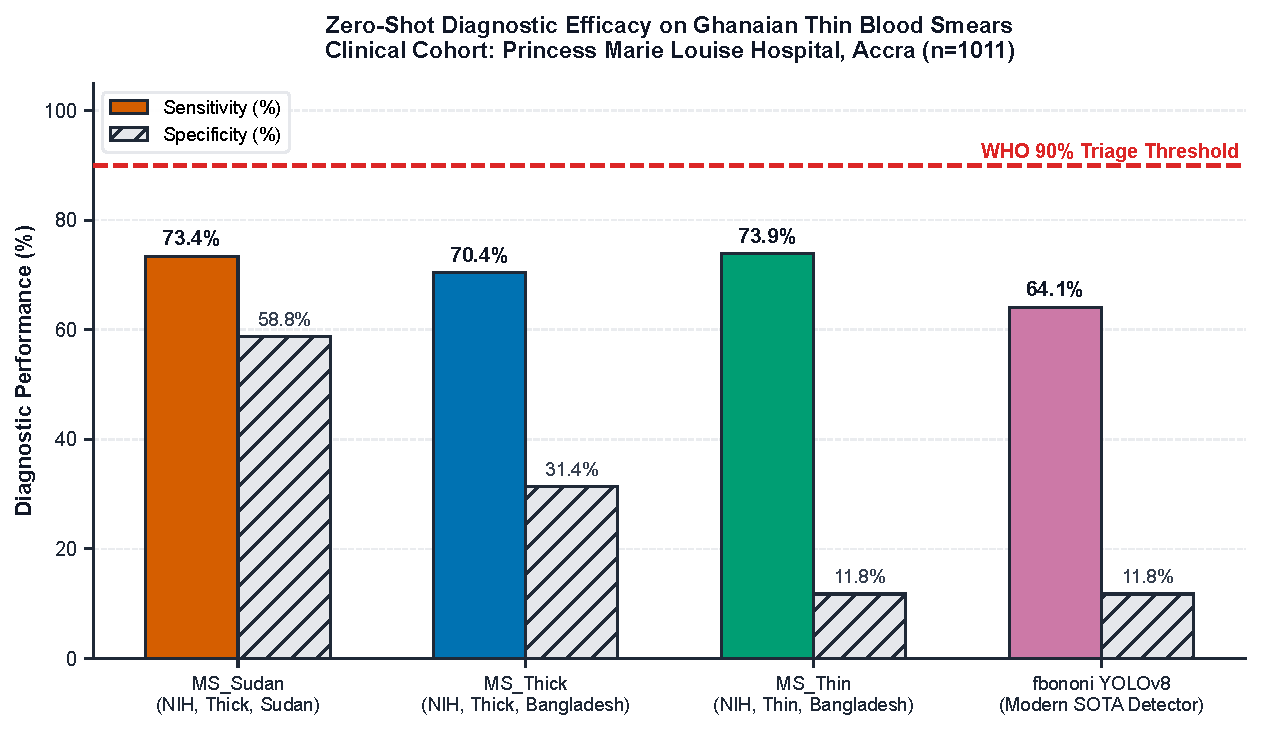
\includegraphics[width=\linewidth]{figures/03_thin_smears/fig_thin_sensitivity_comparison.pdf}
\caption{\textbf{Dual Diagnostic Performance (Sensitivity and Specificity) on Ghanaian Thin Blood Smears ($n=1,011$).} Paired bar chart displaying sensitivity on confirmed parasitized slides ($n=960$; solid colored bars) and specificity on uninfected negative control slides ($n=51$; hatched neutral bars). The crimson dashed line indicates the WHO 90\% clinical sensitivity benchmark \cite{who2016malaria}.}
\label{fig:thin_sensitivity}
\end{figure}

\begin{figure}[htbp]
\centering
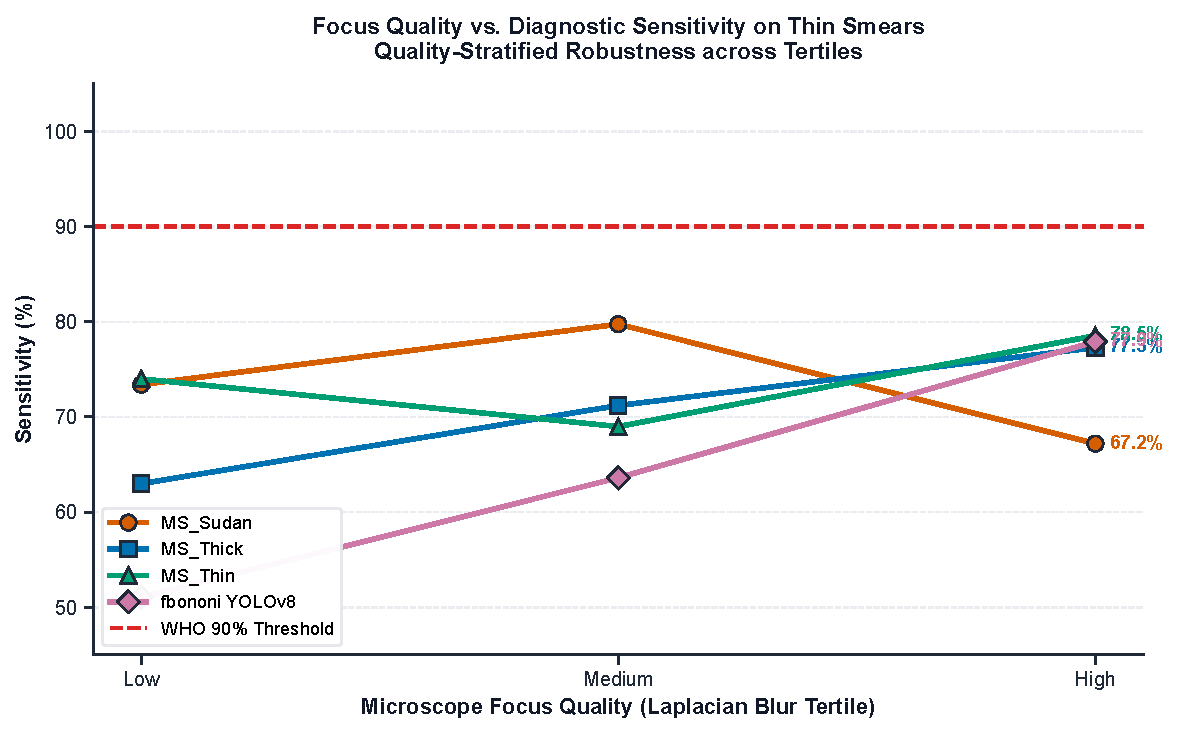
\includegraphics[width=\linewidth]{figures/03_thin_smears/fig_thin_quality_sensitivity_lines.pdf}
\caption{\textbf{Optical Blur Robustness on Thin Blood Smears across Focus Quality Strata.} Diagnostic sensitivity across focus blur tertiles on Ghanaian thin smears ($n=1,011$). Demonstrates differential sensitivity collapse under optical blurring when individual red blood cell borders and intracellular ring-stage trophozoites lose morphological definition.}
\label{fig:thin_quality}
\end{figure}

\begin{figure*}[htbp]
\centering
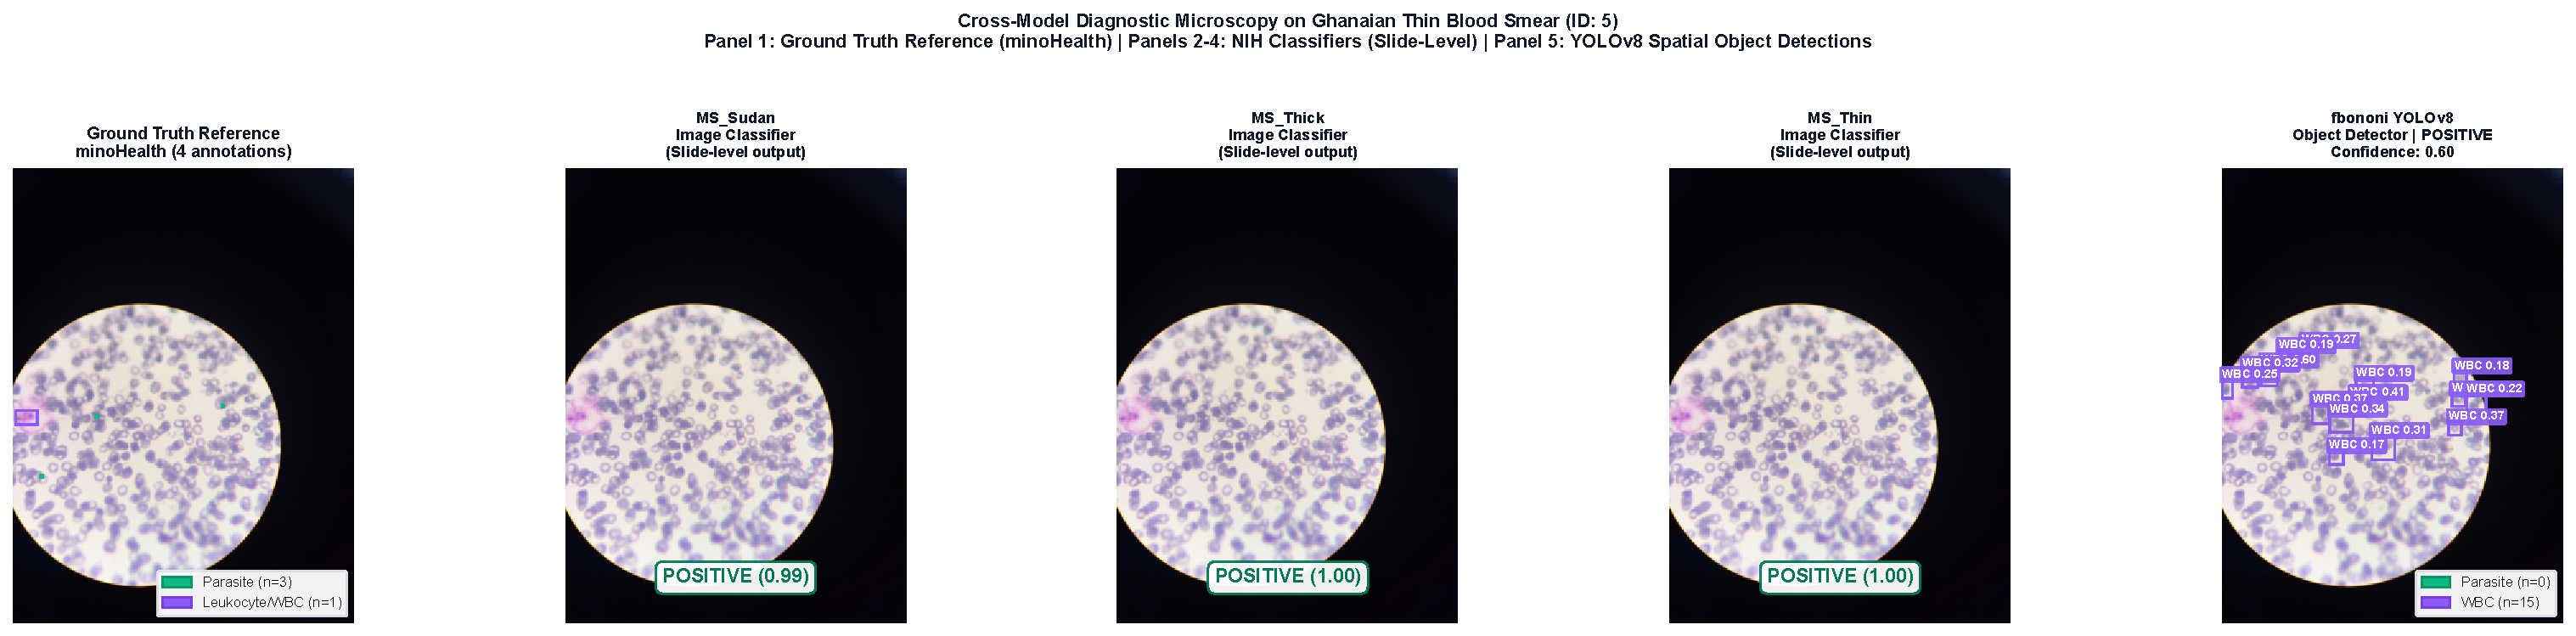
\includegraphics[width=\textwidth]{figures/03_thin_smears/fig_thin_crossmodel_panel.pdf}
\caption{\textbf{Five-Panel Cross-Model Diagnostic Field Inspection on a Representative Ghanaian Thin Smear (Slide ID: 112).} Micrograph with 23 verified ground truth annotations (22 \textit{Plasmodium} parasites and 1 leukocyte). Panel 1 displays ground truth bounding boxes annotated by minoHealth AI Labs expert microscopists (emerald green: parasites; royal violet: leukocytes). Panels 2--4 show whole-slide binary decisions by the NIH MalariaScreener architectures (Sudan, Thick, and Thin) with floating status badges indicating slide-level confidence; these models produce no spatial bounding boxes. Panel 5 displays spatial detections by YOLOv8 with predicted bounding boxes and detected box counts (5 parasites, 1 leukocyte).}
\label{fig:thin_crossmodel_panel}
\end{figure*}

\subsection{Architectural Divergence under Modality Transfer: Object Detectors vs. Whole-Slide Classifiers}
A crucial empirical discovery is the sharp architectural divergence between model families when transferred across slide preparation modalities. While whole-slide MobileNetV2 classifiers proved stable or even slightly improved across modalities---\texttt{MS\_Sudan} increased sensitivity from 66.92\% on thick smears to 73.44\% on thin smears ($+6.52\%$), \texttt{MS\_Thick} increased from 66.66\% to 70.42\% ($+3.76\%$), and \texttt{MS\_Thin} shifted only from 75.73\% to 73.85\% ($-1.88\%$)---the spatial object detector suffered a catastrophic performance cliff. Specifically, \texttt{fbononi\_YOLOv8} collapsed from \textbf{87.43\% sensitivity on thick smears down to 64.06\% on thin smears}---a direct \textbf{23.37 percentage-point drop} (two-tailed Fisher's exact test $\text{OR} = 3.90$, $p = 5.45 \times 10^{-54}$).

This asymmetric failure reflects the distinct visual representations required by the two modalities: whole-slide classifiers evaluate diffuse color distributions and high-level texture, which remain partially preserved across preparations. In contrast, object detectors trained on thick smears learn to localize isolated Giemsa chromatin dots suspended against an amorphous, dehemoglobinized background. When applied to thin smears (Fig.~\ref{fig:thin_crossmodel_panel}), intracellular \textit{P. falciparum} rings are physically enclosed within intact biconcave red blood cells; the detector fails to differentiate faint intra-erythrocytic parasite cytoplasm from the central pallor of normal erythrocytes, resulting in extensive missed detections.

\begin{table}[htbp]
\caption{Diagnostic Sensitivity Across Laplacian Focus Quality Strata}
\label{tab:quality_strata}
\centering
\begin{tabular}{llccc}
\toprule
\textbf{Smear} & \textbf{Model Architecture} & \textbf{Low Focus} & \textbf{Medium Focus} & \textbf{High Focus} \\
\midrule
Thick & \texttt{MS\_Sudan} & 70.96\% & 65.02\% & 63.97\% \\
Thick & \texttt{MS\_Thick} & 67.63\% & 62.22\% & 69.78\% \\
Thick & \texttt{MS\_Thin} & 68.07\% & 78.36\% & 82.24\% \\
Thick & \texttt{fbononi\_YOLOv8} & 86.40\% & 87.51\% & 88.58\% \\
\midrule
Thin & \texttt{MS\_Sudan} & 65.50\% & 81.34\% & 68.99\% \\
Thin & \texttt{MS\_Thick} & 67.50\% & 64.93\% & 78.21\% \\
Thin & \texttt{MS\_Thin} & 81.50\% & 65.92\% & 78.49\% \\
Thin & \textbf{\texttt{fbononi\_YOLOv8}} & \textbf{52.00\%} & \textbf{58.21\%} & \textbf{77.37\%} \\
\bottomrule
\end{tabular}
\end{table}

\subsection{Optical Quality Stratification and Blur Collapse}
Table~\ref{tab:quality_strata} and Figs.~\ref{fig:thick_quality} and \ref{fig:thin_quality} report sensitivity stratified across optical focus tertiles. On thin blood smears, \texttt{fbononi\_YOLOv8} demonstrated an acute blur vulnerability: sensitivity dropped from \textbf{77.37\% in high-focus fields down to 52.00\% in low-focus fields}---a \textbf{25.37 percentage-point collapse}. 
When microscope focus drifts slightly, the delicate hair-like chromatin loops of early \textit{P. falciparum} rings blur into the red cell cytoplasm, completely escaping spatial detection.

\section{Clinical Deployment Safety Translation}
Translating these empirical findings into clinical deployment guidelines for Ghana and West Africa yields three mandatory deployment safety imperatives:

\subsection{The False-Positive Overprescription Crisis}
Deploying models with 11.76\% specificity in endemic primary care clinics presents a severe public health hazard. An 88.24\% false-positive rate results in massive overprescription of Artemisinin-based Combination Therapies (ACTs) to non-malarial febrile patients. This clinical practice carries two disastrous consequences: (1) it rapidly accelerates the selection of artemisinin-resistant \textit{Plasmodium falciparum} mutations in West Africa, and (2) it creates cognitive closure, preventing clinicians from investigating and treating the true underlying etiology of pediatric fever (e.g., bacterial sepsis, meningitis, or pneumonia), thereby increasing preventable mortality.

\subsection{Mandatory Pre-Inference Focus Quality Gating}
Because spatial object detectors suffer up to a 25.37 percentage-point drop in sensitivity under optical defocus, clinical smartphone diagnostic software must not permit unconstrained inference. We mandate that mobile diagnostic applications integrate real-time circular FOV Laplacian focus gating: if $\sigma_{\text{Laplace}}^2 < 12.0$, the software must reject the frame and guide the health worker to adjust the microscope fine-focus knob prior to acquisition.

\subsection{Requirement for African Regional Domain Calibration}
The 5.0-fold specificity advantage and 2.14$\times$ reduction in false-positive rate demonstrated by \texttt{MS\_Sudan} over Asian-trained models confirms that local reagent chemistry, Giemsa formulation, and patient hematological characteristics create a pronounced regional domain shift. AI diagnostic systems must not be deployed in sub-Saharan Africa solely on the basis of high validation scores reported on Asian or European cohorts. Health ministries and regulatory agencies (e.g., the Ghana Food and Drugs Authority) must mandate localized clinical validation and regional calibration before certifying automated diagnostic algorithms.

\section{Limitations}
This empirical benchmark has several limitations:
\begin{enumerate}
    \item \textbf{Sample Imbalance in Negative Controls}: While the clinical dataset is extensive ($N = 4,056$ micrographs), uninfected negative control fields are heavily constrained in the thick-smear cohort ($n=11$ validly evaluated). Consequently, thick-smear specificity estimates carry substantial statistical uncertainty (confidence intervals spanning 35--50 percentage points) and represent exploratory estimates rather than definitive clinical metrics. Thin-smear negative controls ($n=51$) provide stronger statistical power (Fisher's exact test $p < 0.0001$), but future evaluations should prioritize larger prospective negative cohorts.
    \item \textbf{Single-Center Clinical Scope}: All micrographs were acquired at Princess Marie Louise Children's Hospital in Accra. Although capturing an authentic West African clinical distribution, multi-center studies across rural and peripheral district facilities in different ecological zones of Ghana are required to evaluate broader transportability.
    \item \textbf{Fixed Operational Detection Threshold}: The YOLOv8 detector was evaluated at its pre-configured operational detection threshold ($\tau_{\text{det}} = 0.15$). While receiver operating characteristic (ROC) threshold optimization could alter sensitivity-specificity trade-offs, our zero-shot mandate strictly evaluates off-the-shelf deployment readiness without local parameter tuning.
\end{enumerate}

\section{Conclusion}
This study provides the first comprehensive empirical evaluation of zero-shot cross-domain generalization for deep learning malaria models on Ghanaian clinical blood smear data ($N = 4,056$). We show that models trained outside Africa suffer substantial sensitivity gaps, fail to meet WHO triage criteria, and exhibit alarming false-positive rates on uninfected slides. By uncovering the African Regional Advantage, the Architectural Divergence under Modality Transfer, and the Optical Blur Collapse, this benchmark establishes reproducible empirical evidence and concrete deployment-safety standards to ensure safe, effective clinical AI adoption in sub-Saharan Africa.

\section*{Acknowledgment}
The author thanks the clinical microscopists and laboratory personnel at Princess Marie Louise Children's Hospital in Accra, Ghana, as well as the researchers at minoHealth AI Labs and Makerere AI Lab who curated the open Lacuna Malaria Dataset.

\bibliographystyle{IEEEtran}
\bibliography{references}

\end{document}
